\documentclass{stdlocal}
\begin{document}
\section{Pseudorandom Number Generators} % (fold)
\label{sec:pseudorandom_number_generators}
  \subsection{Random Sequences}
  In the section \ref{sub:stochastics} the theory of probability was introduced to make an examination of randomness possible.
  Randomness is a difficult concept and drives many philosophical discussions.
  According to \textcite{volchan2002} and \textcite[\ppno~10-11]{kneusel2018}, humans have a bad intuition concerning the outcome of random experiments.
  But for our purposes, it would suffice to find a formal mathematical definition applicable to RNGs.
  However, such a formal concept, which is also widely accepted and unique, has not been found yet \autocite{volchan2002}.

  The first problem about randomness is the word itself.
  It is unclear and vague because there is no intentional application.
  To be more specific, we will observe randomness in form of random sequences of real numbers.
  But as stated in \textcite{volchan2002} the question if a sequence is random decides at infinity.
  As long as we are only observing finite sequences, we cannot decide if such a sequence is the outcome of a truly random experiment or the result of a non-random algorithm.
  Following his explanation, \citeauthor{volchan2002} makes it clear that typical characterizations of a random sequence are closely associated with noncomputability.
  So even if we would be able to algorithmically produce an infinite amount of numbers, the resulting sequence could not be seen as truly random.
  A modified version of this idea which is easier to understand is given in \textcite{kneusel2018}, where a sequence of values $(x_n)_{n\in\setNatural}$ is truly random if there exists no algorithm such that for all $n\in\setNatural$ the value $x_{n+1}$ can be computed as a function of all $x_i$ with $i\in\setNatural$ and $i\leq n$.
  Put more simply, knowing finitely many elements of a truly random sequence does not enable us to predict the next values within a computer.
  Furthermore, the question if a sequence is random cannot be decided by an algorithm.
  Hence, the existing formal concepts for truly random sequences are not applicable to computer systems.
  Instead, \citeauthor{volchan2002} proposed a more pragmatic principle: \textquote[\cite{volchan2002}]{if it acts randomly, it is random} --- the use of pseudorandom sequences.

  % As a result, we will not use a formalized concept of randomness.
  A computer is only capable of using finite sequences of values and for the development of RNGs, it is enough to measure and compare different properties of truly random sequences to a sequence of real numbers.
  For this, we rely on probability theory and first define an abstract random sequence drawn from a random experiment.
  The definition will use realizations of random variables to model the samples of a random experiment.
  We make sure that these variables are identically and independently distributed (iid).
  This makes analyzing other sequences simpler and imposes no boundary because every important distribution can be generated out of iid random variables \autocite[\ppno~81-111]{kneusel2018}.

  \begin{definition}[Random Sequence]
    Let $I$ be a countable index set and $(X_n)_{n\in I}$ be a sequence of iid real-valued random variables.
    Then a realization of $(X_n)_{n\in I}$ is called a random sequence.
  \end{definition}
  % A system which generates an arbitrarily long abstract random sequence is called a true random number generator (TRNG).
  Generating a truly random sequence in a deterministic computer system is impossible.
  An RNG which is able to generate such a sequence is called a true random number generator (TRNG) and is typically implemented as a device drawing random samples from an essentially non-deterministic physical process, like temperature fluctuations \autocite{intel-drng}.
  % subsection random_and_pseudorandom_sequences (end)

  % \subsection{Random and Pseudorandom Number Generators} % (fold)
  % \label{ssub:random_and_pseudorandom_number_generators}
  \subsection{Pseudorandom Sequences}
  The given abstract definition of a random sequence in terms of probability theory helps to assess the randomness properties of a given sequence produced by a computer.
  Typically, a computer-generated sequence which fulfills various conditions about randomness will be called a pseudorandom sequence.
  The respective structure and algorithm which produced the sequence is then called a PRNG.

  For computer programming and simulations, the usage of a TRNG would introduce severe disadvantages in contrast to a PRNG.
  A PRNG generates numbers according to a deterministic algorithm.
  Therefore its output cannot be seen as truly random.
  But concerning program verification, debugging, and the comparison of similar systems, the reproducibility of results is essential \autocite{lecuyer2015}.
  A truly random sequence produced by physical devices, such as thermal noise diodes or photon trajectory detectors, is not reproducible and can therefore not be conveniently used for mathematical and physical simulations \autocite{lecuyer2015}.
  According to \textcite{lecuyer2015}, a given simulation should produce the same results on different architectures for every run.
  This property becomes even more important if parallel generation of random numbers with multiple streams is taken into account.
  Additionally, considering the performance of random number generation PRNGs tend to be much faster than TRNGs \autocite{intel-drng}.
  Thus, especially for Monte Carlo methods, PRNGs are a key resource for computer-generated random numbers \autocite{bauke2007}.

  For a detailed discussion about its mathematical properties, design, and implementation, the concept of a PRNG has to be formalized.
  In this thesis, we use the following slightly modified variation of \citeauthor{lecuyer1994}'s definition \autocite{lecuyer1994,lecuyer2015,barash2017,bauke2007}.
  It assumes a finite set of states and a transition function which advances the current state of the PRNG by a recurrence relation.
  For the output, a finite set of output symbols and a generator function which maps states to output symbols is chosen.
  As of \textcite{bauke2007}, almost all PRNGs produce a sequence of numbers by a recurrence.
  Hence, the given formalization is widely accepted and builds the basis for further discussions about pseudorandom numbers \autocite{lecuyer1994,lecuyer2015,barash2017,bauke2007}.

  \begin{definition}[Pseudorandom Number Generator (PRNG)]
    Let $\mathscr{G}\define (S,T,U,G)$ be a tuple consisting of a non-empty, finite set of states $S$, a transition function $\function{T}{S}{S}$, a non-empty, finite set of output symbols $U$ and an output function $\function{G}{S}{U}$.
    In this case $\mathscr{G}$ is called a PRNG.
  \end{definition}
  Given a PRNG and a seed value as an initial state, producing a sequence of pseudorandom numbers can be done by periodically applying the transition function on the current state and then extracting the output through the generator function \autocite{barash2017,lecuyer1994,lecuyer2015}.
  Here, we will use this method as the generalization of a pseudorandom sequence.
  Figure \ref{fig:scheme-pseudorandom-sequence} shows this process schematically.

  \begin{definition}[Pseudorandom Sequence of PRNG]
    Let $\mathscr{G}\define (S,T,U,G)$ be a PRNG and $s_0\in S$ be the initial state, also called the seed value.
    The respective sequence of states $(s_n)_{n\in\setNatural}$ in $S$ is given by the following equation for all $n\in\setNatural$.
    \[
      s_{n+1} \define T(s_n)
    \]
    The sequence $(u_n)_{n\in\setNatural}$ in $U$ given by the following expression for all $n\in\setNatural$ is then called the respective pseudorandom sequence of $\mathscr{G}$ with seed $s_0$.
    \[
      u_n \define G(s_n)
    \]
  \end{definition}
  \begin{figure}
    \center
    % \begin{minipage}[b]{0.5\textwidth}
    % \begin{alignat*}{3}
    %   s_0 \xrightarrow{T} &s_1 \xrightarrow{T} &&s_2 \xrightarrow{T} &&\ldots \\
    %   G &\downarrow &&\downarrow \\
    %   &u_1 &&u_2 &&\ldots
    % \end{alignat*}
    % \end{minipage}
    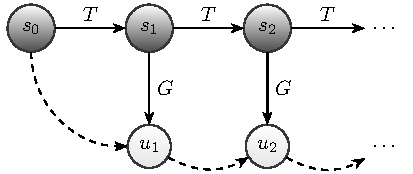
\includegraphics[width=0.5\textwidth]{figures/sequence_generation_scheme.pdf}
    \caption[Generation of a Pseudorandom Sequence]{%
      Generation of a pseudorandom sequence for a given PRNG $\mathscr{G}\define (S,T,U,G)$ and seed value $s_0\in S$.
      The internal state is advanced by the transition function $T$ through a recurrence relation.
      To get an output value for the pseudorandom sequence the generator function $G$ is used.
    }
    \label{fig:scheme-pseudorandom-sequence}
  \end{figure}
  In the definition we have used a recursive formulation.
  For theoretical discussions and the initialization of multiple streams of pseudorandom numbers an explicit variation seems to be more adequate.
  The following lemma will be given without a proof, but it can be shown by mathematical induction.

  \begin{lemma}[Explicit Formulation of Pseudorandom Sequence]
  \label{lemma:explicit-formulation-pseudorandom-sequence}
    Let $\mathscr{G}\define (S,T,U,G)$ be a PRNG and $s_0\in S$ its initial state.
    Then the respective pseudorandom sequence $(u_n)_{n\in\setNatural}$ is given by the following formula for all $n\in\setNatural$.
    \[
      u_n = G\circ T^{n}(s_0)
    \]
  \end{lemma}

  \subsection{Explanation of the Concept}
  Using a TRNG in a computer system is like consulting an oracle \autocite{mueller2012}.
  We are calling a function with no arguments which returns a different value for every call.
  Let $(u_n)_{n\in\setNatural}$ be the respective pseudorandom sequence of a PRNG $\mathscr{G}$ with a given seed.
  Then in a computer $\mathscr{G}$ can be interpreted as a function with no parameters which produces the pseudorandom sequence $(u_n)_{n\in\setNatural}$ in the following way.
  Hereby, we understand $\leftarrow$ as the assignment operator that assigns a value given on the right-hand side to the variable given on the left-hand side.
  \[
    u_1 \leftarrow \mathscr{G}()
    \separate
    u_2 \leftarrow \mathscr{G}()
    \separate
    u_3 \leftarrow \mathscr{G}()
    \separate
    \ldots
  \]
  A PRNG has to artificially model this behavior by an internal state.
  Every function call must change this state according to the transition function.
  Consequently, if a PRNG should be used as an oracle in that sense, the set of states and the transition function in its definition are obligatory.

  It will be shown that the number of different states a PRNG can reach greatly affects the randomness of a respective pseudorandom sequence.
  A larger set of states is not a guarantee that the output of a PRNG will look more like a truly random sequence, but at least gives the opportunity to mask its deterministic nature very well \autocite{oneill2014}.
  Therefore the number of states in general is much bigger than the number of different outputs.
  Through the usage of output symbols together with a generator function a PRNG can take advantage of a large set of states while returning only a few different values.
  This idea has two important implications.
  A generator function which shrinks the set of states to a smaller space of output symbols makes the PRNG less predictable and more secure \autocite{oneill2014}.
  The generator function would not be bijective and as a result we as consumers would not be able to draw conclusions about the current state of the PRNG based on its given output.
  Both properties are highly appreciated because they mimic the behavior of TRNGs.
  Hence, the set of output symbols and the generator function in the definition of PRNGs is as important as the set of states and the transition function.

  In the majority of cases, the transition function $T$ of a PRNG $\mathscr{G}$ should be injective \autocite{lecuyer1994,lecuyer2015,widynski2019,oneill2014}.
  Because we have a finite set of states this is equivalent to the proposition that $T$ is a permutation and therefore bijective \autocite[\ppno~201-202]{waldmann2017}.
  The property makes sure that every state is reached at a certain point in a sequence without introducing bias in the resulting distribution \autocite{oneill2014}.
  The generator function $G$ cannot be a permutation but should not distort the distribution either.
  Hence, a uniform function which maps to every output value the same number of input values is a perfect candidate \autocite{oneill2014}.

  \subsection{Randomization}
  The goal of PRNGs is to imitate the properties of TRNGs as much as possible \autocite{lecuyer1994} and at the same time retain executability by a computer system and reproducibility for a given seed \autocite{lecuyer2015}.
  These restrictions make a pseudorandom sequence completely predictable and characterizable by its seed.
  So until now, we have not introduced any kind of randomness to the definition of a PRNG.
  But to extend the process of generating a pseudorandom sequence with true randomness, the seed will be chosen to be a truly random number produced by a TRNG.
  \textcite{lecuyer1994} states that receiving such a seed is much less work and more reasonable than acquiring a long sequence of truly random values.
  A generator with a truly random seed can be seen as an extensor of randomness.
  Even today, \citeauthor{intel-drng} uses hardware-implemented PRNGs repeatedly seeded by a high-quality entropy source in their CPUs to provide a high-performance hardware module for producing random numbers with good statistical quality and protection against attacks \autocite{intel-drng}.

  \begin{definition}[Randomized Pseudorandom Sequence]
    Let $\mathscr{G}\define (S,T,U,G)$ be a PRNG and $X$ be an $S$-valued random variable with distribution $P_X$.
    Then the randomized pseudorandom sequence $(X_n)_{n\in\setNatural}$ of $\mathscr{G}$ with respect to $P_X$ is defined by the following expression for all $n\in\setNatural$.
    \[
      X_n \define G \circ T^n \circ X
    \]
  \end{definition}
  As with abstract random sequences, a truly random seed value is again modeled by a realization of the random variable $X$.
  As a result, the randomized pseudorandom sequence becomes a sequence of random variables which all depend on $X$.
  For the definition the explicit formulation in lemma \ref{lemma:explicit-formulation-pseudorandom-sequence} was used.
  Typically, the distribution of seed values $P_X$ is chosen so that it is uniformly distributed in a certain subset of $S$ \autocite{matsumoto1998,oneill2014,lecuyer1994,lecuyer2015,bauke2007}.
  This makes sure that no bias will be introduced by the randomization.

  % \subsection{Distributions}

  \subsection{Limitations and Mathematical Properties}
  As was already discussed, PRNGs have certain advantages in comparison with TRNGs.
  But they are also yielding essential and intrinsic limitations.
  From the previous subsection, it becomes clear that all the samples of a randomized pseudorandom sequence are not stochastically independent.
  In general, this means the output of a PRNG can consist of certain regular patterns or artifacts \autocite{lecuyer1994,oneill2014}.
  In \textcite{lecuyer1994} these artifacts are also called the lattice structure.
  % Such patterns can be visualized by so-called randograms.
  % The typical approach to prevent the user of a PRNG to observe this dependence is to construct a complex generator function that scrambles the output.
  For applications that are using a large amount of random numbers, such patterns will introduce bias in the evaluated outputs.
  Hence, we will discuss a few mathematical properties a PRNG should fulfill to reduce the lattice structure as much as possible.

  \subsubsection*{Periodicity}
  Since the set of states in a PRNG is finite, every respective pseudorandom sequence has to be periodic or ultimately periodic \autocite{lecuyer1994,bauke2007}.
  First, a rigorous definition of this concept should be given.

  \begin{definition}[Periodic and Ultimately Periodic Sequences]
    Let $U$ be a non-empty set and $(u_n)_{n\in\setNatural}$ be a sequence in $U$.
    Assume there exist $ρ,τ\in\setNatural$ such that for all $n\in\setNatural_0$ the following holds.
    \[
      u_{τ+n+ρ} = u_{τ+n}
    \]
    Then $(u_n)$ is called ultimately periodic.
    The smallest possible values for ρ and τ, such that the equation holds, are called period and transient respectively.
     % with period ρ and transient τ.
    In particular, if τ equals to $1$ we call $(u_n)$ periodic with period ρ.
  \end{definition}
  This means an ultimately periodic sequence will be periodic after it has reached its transient.
  Every periodic sequence is therefore ultimately periodic but not vice versa and as another consequence, the given concept is more general than the typical one of a periodic sequence.
  Please note that the values for ρ and τ are not unique.
  Let $ρ^*$ be the period and $τ^*$ be the transient.
  Then the equation given in the above definition holds for all the values of ρ and τ with respect to $m\in\setNatural$ and $n\in\setNatural_0$ in the following sense.
  \[
    ρ = mρ^*
    \separate
    τ = τ^* + n
  \]
  Choosing the minimal values allows us to talk about a unique transient and a unique period.
  In the following lemma we show the application of the definition to pseudorandom sequences.
  The proof can be found in appendix \ref{sec:proofs}.

  \begin{lemma}[Pseudorandom Sequences are Ultimately Periodic]
  \label{lemma:pseudorandom-sequences-periodicity}
    Let $\mathscr{G}\define (S,T,U,G)$ be a PRNG and $s_0\in S$ its initial state.
    Then the respective pseudorandom sequence $(u_n)_{n\in\setNatural}$ is ultimately periodic.
    In this case, for the period ρ and the transient τ the following holds.
    \[
      1 \leq ρ + τ - 1 \leq \# S
    \]
    In particular, if $T$ is bijective $(u_n)$ will be periodic.
  \end{lemma}
  % \begin{proof}[Lemma~\ref{lemma:pseudorandom-sequences-periodicity}]
  %   Let $(s_n)_{n\in\setNatural}$ be the respective sequence of states and $N\define \# S$ the number of different states.
  %   $T$ maps all elements of $S$ to at most $N$ other elements of $S$.
  %   Therefore at least the element $s_N$ has to be mapped to an element $s_k$ for $k\in\setNatural$ with $k\leq N$ which was already reached.
  %   % Hence, there exist $n,k\in\setNatural$ with $k\leq n\leq N$ such that $T(s_n) = s_k$.
  %   Hence, we conclude the following.
  %   \[
  %     \exists n,k\in\setNatural, k\leq n\leq N: \quad T(s_n) = s_k
  %   \]
  %   % Assume $T$ maps $s_n$ to a state $s_k$ with $k\in\setNatural$ and $k < n$.
  %   We choose $n$ and $k$ appropriately and define the following values.
  %   \[
  %     ρ \define n - k + 1
  %     \separate
  %     τ \define k
  %   \]
  %   Now let $i\in\setNatural_0$ be arbitrary and apply the definition.
  %   We get the following chain of equations which show that $(u_n)$ is ultimately periodic.
  %   \[
  %     \begin{aligned}
  %       u_{τ+i+ρ} &= u_{n+1+i} = G \circ T^{n+1+i}(s_0) = G \circ T^i\circ T^{n+1}(s_0) \\
  %       &= G \circ T^i(s_k) = G \circ T^i \circ T^k(s_0) = G \circ T^{i+k}(s_0) = u_{k+i} = u_{τ+i}
  %     \end{aligned}
  %   \]
  %   The inequality can be shown by directly inserting the values into the definition.
  %   \[
  %     1 \leq ρ + τ - 1 = n \leq N = \# S
  %   \]
  %   This proofs the given lemma.
  % \end{proof}
  Thus, every pseudorandom sequence will repeat itself after it reached a certain point.
  The period and the transient are greatly affected by the number of states and the transition function of the PRNG.
  To get a better insight, we will examine the following idealized examples with different transition functions.
  Let $\mathscr{G}\define (S,T,U,G)$ be a PRNG defined as follows.
  \[
    S \define U \define \setInteger_4
    \separate
    G \define \identity
  \]
  For a seed $s_0 \in S$ the respective pseudorandom sequence $(u_n)_{n\in\setNatural}$ with period ρ and transient τ will be shown in the following way.
  Hereby, all elements of the sequence up to the end of the first period are written consecutively and the periodic part is marked by an overline.
  \[
    (u_n) = u_1\ldots u_{τ-1} \overline{u_τ\ldots u_{τ+ρ-1}}
  \]
  To the left of the examples, a scheme of their respective transition function is displayed to make the originating sequences together with their periods and transients more understandable.
  The boxes are used in place of the set of states $S$ whereas arrows characterize the transition function $T$.

  \medskip
  \begin{minipage}{0.2\textwidth}
    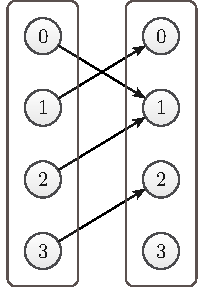
\includegraphics[width=\textwidth]{figures/periodicity_example_a.pdf}
  \end{minipage}
  \hfill
  \begin{minipage}{0.73\textwidth}
    \[
      T(x) \define
      \begin{cases}
        1 &: x \in \set{0,2}{} \\
        0 &: x = 1 \\
        2 &: x = 3
      \end{cases}
      \separate
    % \]
    % \[
      (u_n) =
      \begin{cases}
        \overline{10} &: s_0 \in \set{0,2}{} \\
        \overline{01} &: s_0 = 1 \\
        2\overline{10} &: s_0 = 3
      \end{cases}
    \]
  \end{minipage}
  \medskip
  \par
  \noindent
  The first example shows a transition function which is not bijective and does not map any element of $S$ to itself.
  Hence, in all cases we get a period of $2$.
  The transient varies between $1$ and $2$ and depends on the seed value.

  \medskip
  \begin{minipage}{0.2\textwidth}
    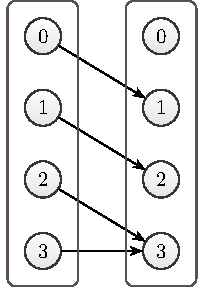
\includegraphics[width=\textwidth]{figures/periodicity_example_b.pdf}
  \end{minipage}
  \hfill
  \begin{minipage}{0.73\textwidth}
    \[
      T(x) \define
      \begin{cases}
        x + 1 &: x < 3 \\
        3 &: x = 3
      \end{cases}
    % \]
    % \[
    \separate
      (u_n) =
      \begin{cases}
        12\overline{3} &: s_0 = 0 \\
        2\overline{3} &: s_0 = 1 \\
        \overline{3} &: s_0 \geq 2 \\
      \end{cases}
    \]
  \end{minipage}
  \medskip

  \noindent
  In the second example, again a non-bijective transition function is used.
  This time the value $3$ is mapped to itself and as a consequence the period for all possible sequences is $1$.
  As before, the transient varies with respect to the seed value.

  \medskip
  \begin{minipage}{0.2\textwidth}
    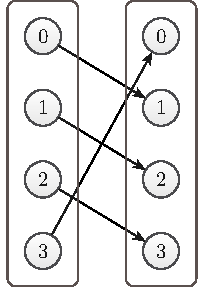
\includegraphics[width=\textwidth]{figures/periodicity_example_c.pdf}
  \end{minipage}
  \hfill
  \begin{minipage}{0.73\textwidth}
    \[
      T(x) \define x + 1 \mod 4
    % \]
    % \[
    \separate
      (u_n) =
      \begin{cases}
        \overline{1230} &: s_0 = 0 \\
        \overline{2301} &: s_0 = 1 \\
        \overline{3012} &: s_0 = 2 \\
        \overline{0123} &: s_0 = 3
      \end{cases}
    \]
  \end{minipage}
  \medskip

  \noindent
  In the third example, a bijective transition function is used.
  The period is maximized and reaches the number of states.
  In all cases the transient is $1$ and as a result all sequences are periodic.

  \medskip
  \begin{minipage}{0.2\textwidth}
    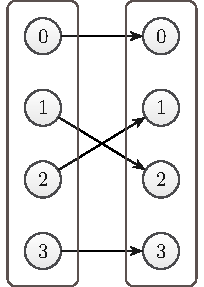
\includegraphics[width=\textwidth]{figures/periodicity_example_d.pdf}
  \end{minipage}
  \hfill
  \begin{minipage}{0.73\textwidth}
    \[
      T(x) \define
      \begin{cases}
        x &: x \in \set{0,3}{} \\
        2 &: x = 1 \\
        1 &: x = 2
      \end{cases}
    % \]
    % \[
    \separate
      (u_n) =
      \begin{cases}
        \overline{0} &: s_0 = 0 \\
        \overline{21} &: s_0 = 1 \\
        \overline{12} &: s_0 = 2 \\
        \overline{3} &: s_0 = 3
      \end{cases}
    \]
  \end{minipage}
  \medskip

  \noindent
  The last example shows again a bijective transition function $T$.
  The transient is again always $1$ and all possible pseudorandom sequences are purely periodic.
  But this time, $T$ maps the values $0$ and $3$ to themselves.
  Hence, the period becomes dependent on the initial value and differs between the smallest possible value $1$ and $2$.\\
  The periodic behavior of pseudorandom sequences greatly constrains the possible randomness of a PRNG.
  Especially for simulations, using a PRNG which is repeating itself while in use introduces unwanted regularities resulting in an incorrect output.
  As a consequence, developers of PRNGs try to construct a large period by adjusting the number of states and the transition function.
  For example, the MT19937 is a PRNG with an extremely large period of $2^{19937}-1$ if not used with a seed value of zero \autocite{matsumoto1998}.
  The use of a bijective transition function is not enough to ensure the maximal period.
  Values that are mapped to themselves result in the smallest possible period even if the transient of the sequence could be large.
  Especially for linear PRNGs that are mapping $0$ to itself, developers tend to exclude such states from the seeding process to always obtain the maximal period \autocite{marsaglia2003,blackman2019}.
  As a counter-example, the so-called \enquote{Middle Square RNG} which was developed by Von Neumann in the early days of computer science should be named \autocites[\ppno~12-15]{kneusel2018}{widynski2019}.
  This PRNG computed the square of its current state and returned the middle digits as next random number.
  It was well known to suffer from the \enquote{zero mechanism} --- once some digits become zero, all following return values would be zero as well \autocites[\ppno~12-15]{kneusel2018}{widynski2019}.
  So besides a large state space and a bijective transition function, the largest possible permutation cycle should be reached when advancing the state of a PRNG.

  \subsubsection*{Equidistribution}
  Pseudorandom sequences should mimic the behavior of truly random sequences.
  And for that reason, we want them to be uniformly distributed on the set of output values in some sense.
  This property will make it possible to generate every important distribution of random numbers by applying special transformations based on stochastics.
  Such distributions can then be used by Monte Carlo simulations to estimate solutions more efficiently.
  But because we are dealing with actual values instead of random variables, we have to clarify what uniformly distributed means.
  Consequently, we will again rely on probability theory to elaborate on the details without a deeper understanding of randomness \autocite{eisner2019}.
  To be able to always distinct these two different concepts, we will call a sequence of actual values with the desired properties equidistributed.

  \begin{definition}[Equidistributed Sequence]
    Let $U$ be a non-empty, finite set of values and μ be a probability measure on the measurable space $(U,\mathscr{P}(U))$.
    A sequence $(u_n)_{n\in\setNatural}$ in $U$ is equidistributed with respect to μ if for every measurable function $\function{X}{U}{\setReal}$ the following is true.
    \[
      \lim_{n\to\infty} \frac{1}{n} \sum_{k=1}^n X(u_k) = \integral{U}{}{X}{μ}
    \]
    If μ is not specified, we assume it to be the uniform distribution on $U$.
  \end{definition}
  The idea is that every possible output value should essentially be reached the same amount of times when advancing the state.
  For pseudorandom sequences generated by a non-bijective transition function the transient part should be ignored as it can be seen as non-recurring \enquote{warm-up} time.
  Therefore equidistribution will be evaluated at infinity in the sense of a limit.
  Because we wanted to use probability theory to observe randomness, we had to generalize the idea of counting how often different output values would be reached.
  Instead we use arbitrary measurable functions as observables to estimate their expectation value with respect to the given sequence and to compare it to their actual expectation value \autocite{eisner2019}.
  Please note that for our needs we have chosen a finite set of elements to simplify the definition of equidistribution.
  A more general alternative where $U$ has to be a compact metric space with Borel probability measure μ can be found in \textcite{eisner2019}.
  Here, measurable functions are interchanged with continuous functions.
  Because of this, we can further simplify the right-hand side of the definition.
  \[
    \integral{U}{}{X}{μ} = \expect X = \sum_{u\in U} f(u) μ(\set{u}{})
  \]
  To make sure the generalization is working properly, we proof the following lemma in appendix \ref{sec:proofs} which states that, while observing pseudorandom sequences, the relative frequency in one period of an arbitrary element must be given by its probability.

  \begin{lemma}[Equidistributed Pseudorandom Sequences]
  \label{lemma:equidistribution}
    Let $\mathscr{G}\define (S,T,U,G)$ be a PRNG with $s_0\in S$ as its seed value and $(u_n)_{n\in\setNatural}$ the respective pseudorandom sequence with transient τ and period ρ.
    Furthermore, let μ be a probability measure on $(U,\mathscr{P}(U))$.
    Then the following statements are equivalent.
    \begin{enumerate}[label=(\roman*)]
      \item $(u_n)$ is equidistributed with respect to μ.
      \item For all $u\in U$ the following is true.
        \[
          \frac{1}{ρ} \cdot \#\set{n\in\setNatural}{τ\leq n < ρ+τ, u_n = u} = μ(\set{u}{})
        \]
    \end{enumerate}
  \end{lemma}
  % \begin{proof}[Lemma~\ref{lemma:equidistribution} on page \ref{lemma:equidistribution}]
  %   Because $U$ is a finite set, every measurable function $\function{X}{U}{\setReal}$ can be described as a linear combination of characteristic functions with respect to some real coefficients $α_u$ for all $u \in U$ in the following way.
  %   \[
  %     X = \sum_{u\in U} α_u \mathds{1}_{\set{u}{}}
  %   \]
  %   Hence, without loss of generality, it suffices to take only characteristic functions into account.
  %   Let $u\in U$ be arbitrary.
  %   The right-hand side of the definition will then result in the following.
  %   \[
  %     \integral{U}{}{\mathds{1}_{\set{u}{}}}{μ} = μ(\set{u}{})
  %   \]
  %   Applying the characteristic function together with the properties of a periodic sequence to the left-hand side of the definition, looks as follows.
  %   \[
  %     \begin{aligned}
  %       \lim_{n\to\infty} \frac{1}{n} \sum_{k=1}^n \mathds{1}_{\set{u}{}}(u_k)
  %       &= \lim_{n\to\infty} \frac{1}{n} \sum_{k=1}^{τ-1} \mathds{1}_{\set{u}{}}(u_k) + \lim_{n\to\infty} \frac{1}{n}\sum_{k=τ}^{τ+n-1} \mathds{1}_{\set{u}{}}(u_k) \\
  %       &= \frac{1}{ρ} \sum_{k=τ}^{τ+ρ-1} \mathds{1}_{\set{u}{}}(u_k) \\
  %       &= \frac{1}{ρ} \cdot \#\set{n\in\setNatural}{τ\leq n < ρ+τ, u_n = u}
  %     \end{aligned}
  %   \]
  %   This shows the desired equivalence and proofs the lemma.
  % \end{proof}
  Based on this lemma, it directly follows that for equidistributed, pseudorandom sequences with a maximal period the number of different states has to be a multiple of the number of output values.

  \begin{corollary}[Equidistributed Pseudorandom Sequence with Maximal Period]
    Let $\mathscr{G}\define (S,T,U,G)$ be a PRNG with $s_0\in S$ as its initial state and $(u_n)_{n\in\setNatural}$ the respective pseudorandom sequence.
    If $(u_n)$ is equidistributed and periodic with maximal period $\# S$ then the following is true.
    \[
      \exists k\in\setNatural:\quad \# S = k \cdot \# U
    \]
  \end{corollary}
  % The given definition can be directly applied to PRNGs.

  % \begin{definition}[Equidistribution]
  %   Let $\mathscr{G}\define (S,T,U,G)$ be a PRNG and $S_0 \subset S$ a set of seeds.
  %   $\mathscr{G}$ is said to be equidistributed with respect to $S_0$ if for all seeds $s_0 \in S_0$ the respective pseudorandom sequence is equidistributed.
  % \end{definition}
  % A PRNG is called equidistributed if every possible pseudorandom sequence is equidistributed.

  \subsubsection*{Multidimensional Equidistribution}
  In physical problems, we typically have to deal with partial differential equations in many dimensions.
  Finding deterministic, numerical solutions through iterated integrals becomes infeasible due to the resulting degrees of freedom.
  % This is called the \enquote{curse of dimensionality}.
  With the use of Monte Carlo integration, we can overcome this burden so that for high-dimensional problems we are able to reduce the error of the estimated solutions for every iteration much faster.
  % The advantage of using Monte Carlo methods to solve a problem is that through the use of random numbers we are able to overcome the curse of dimensionality.
  % As a consequence, a PRNG should provide random vectors for a different number of dimensions.
  % Typical Monte-Carlo Simulations need to construct random vectors.
  As a consequence, successive pseudorandom numbers generated by a PRNG should be interpretable as a pseudorandom vector.
  But due to the shown dependence of successive values in a pseudorandom sequence, again regular patterns and artifacts can arise which can only be observed by some advanced testing techniques for statistical performance.
  However, a PRNG that is used in more than one dimension should at least provide an equidistribution over all possible multidimensional output values.
  For a rigorous definition of this concept, we will first clarify how to use a pseudorandom sequence as a sequence of pseudorandom vectors.

  \begin{definition}[Corresponding Vector Sequence]
    Let $U$ be a non-empty set of values and $(u_n)_{n\in\setNatural}$ be a sequence in $U$.
    Choose $k\in\setNatural$ and $t\in\setNatural_0$ and define the following for all $n\in\setNatural$.
    \[
      v_n \define (u_i)_{i\in I_n}
      \separate
      I_n \define \set{t + (n-1)k + p}{p\in\setNatural, p \leq k}
    \]
    We call the sequence $(v_n)_{n\in\setNatural}$ in $U^k$ the corresponding $k$-dimensional vector sequence with translation $t$ with respect to $(u_n)$.
  \end{definition}
  Transforming a sequence of values into a sequence of vectors consists of interpreting successive values as coordinates of vectors.
  Figure \ref{fig:vector-sequence-scheme} shows this process schematically.
  \begin{figure}
    \center
    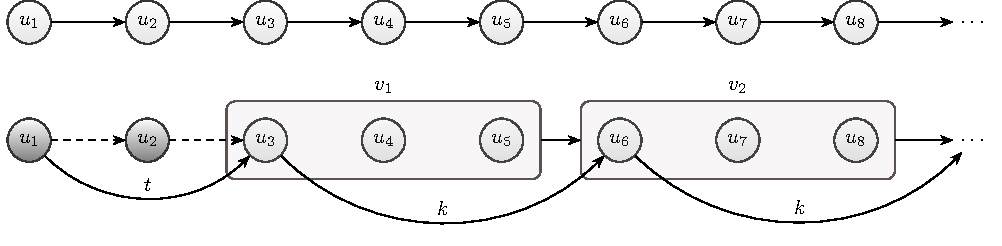
\includegraphics[width=0.9\textwidth]{figures/vector_sequence_scheme.pdf}
    \caption[Corresponding Vector Sequence Scheme]{%
      The upper part of the figure shows a schematic view of an arbitrary sequence of values $(u_n)_{n\in\setNatural}$ in an arbitrary non-empty set $U$.
      The lower part visualizes the corresponding $k$-dimensional vector sequence $(v_n)_{n\in\setNatural}$ with translation $t$, whereby $k=3$ and $t=2$.
      The first two values of $(u_n)$ are skipped due to the translation.
      Afterwards the elements of $(v_n)$, marked through boxes, emerge from interpreting successive values of $(u_n)$ as their coordinates.
    }
    \label{fig:vector-sequence-scheme}
  \end{figure}
  Corresponding vector sequences inherit the property of being ultimately periodic.

  \begin{lemma}[Corresponding Vector Sequences are Ultimately Periodic]
  \label{lemma:vector-sequences-periodicity}
    Let $U$ be a non-empty set of values and $(u_n)_{n\in\setNatural}$ be an ultimately periodic sequence in $U$ with period ρ and transient τ.
    In this case, every corresponding $k$-dimensional vector sequence $(v_n)_{n\in\setNatural}$ with translation $t$ is ultimately periodic with period $ρ'$ and transient $τ'$ defined as follows.
    \[
      ρ' \define \frac{ρ}{\mathrm{gcd}(ρ,k)}
      \separate
      τ' \define \ceilBrackets{\frac{\max(0,τ-1-t)}{k}} + 1
    \]
  \end{lemma}
  % \begin{proof}[Lemma \ref{lemma:vector-sequences-periodicity} on page \ref{lemma:vector-sequences-periodicity}]
  %   Choose $n\in\setNatural_0$ and $i\in\setNatural$ with $i\leq k$ to be arbitrary.
  %   We denote with $v^{(i)}_n$ the $i$.~coordinate of the $n$.~vector.
  %   By definition the following equality holds.
  %   \[
  %     v^{(i)}_{τ' + n + ρ'} = u_{t + (τ'+n+ρ'-1)k + i}
  %   \]
  %   Observing the index, we separate it into three parts.
  %   One for the index, one for the transient one for the period.
  %   \[
  %     t+(τ' + n + ρ' - 1)k + i = \underbrace{(t + τ'k - k + 1)}_{\reverseDefine \tilde{τ}} + \underbrace{(nk + i - 1)}_{\reverseDefine \tilde{n}}  + \underbrace{ρ'k}_{\reverseDefine \tilde{ρ}}
  %   \]
  %   The period part has to be a multiple of the period ρ of $(u_n)$ as can be seen in the following.
  %   Hence, $\tilde{ρ}$ has the property of a period.
  %   \[
  %     \tilde{ρ} = ρ'k = \frac{ρk}{\mathrm{gcd}(ρ,k)} = ρ \frac{k}{\mathrm{gcd}(ρ,k)}
  %   \]
  %   To apply the periodicity of $(u_n)$, the transient part has to be bigger or equal to the transient τ of $(u_n)$.
  %   \[
  %     \tilde{τ} = t + τ'k - k + 1 = 1 + t + k \ceilBrackets{\frac{\max(0,τ-1-t)}{k}} \geq τ
  %   \]
  %   Inserting the results and applying the periodicity of $(u_n)$, we can conclude that the corresponding vector sequence has to be ultimately periodic as well.
  %   \[
  %     v^{(i)}_{τ' + n + ρ'} = u_{\tilde{τ} + \tilde{n} + \tilde{ρ}} = u_{\tilde{τ} + \tilde{n}} = u_{t + (τ' + n - 1)k + i} = v^{(i)}_{τ' + n}
  %   \]
  %   Due to the shown statements, $ρ'$ and $τ'$ are indeed the smallest possible values such that this equation holds and can therefore be denoted as period and transient of $(v_n)$ respectively.
  % \end{proof}
  The given concept shall now be applied to define the equidistribution of a sequence in more than one dimension.
  As a result, the following property, called multidimensional equidistribution, becomes a generalization of equidistribution and quantifies in how many dimensions a PRNG can be used.
  We do not follow the typical definitions from \textcite{matsumoto1998,lecuyer1994}.

  \begin{definition}[Multidimensional Equidistributed Sequence]
    Let $U$ be a non-empty, finite set of values, $k\in\setNatural$ and μ be a probability measure on $\roundBrackets{U^k,\mathscr{P}\roundBrackets{U^k}}$.
    A sequence $(u_n)_{n\in\setNatural}$ in $U$ is $k$-dimensional equidistributed with respect to μ if for all $t\in\setNatural_0$ the corresponding $k$-dimensional vector sequence with translation $t$ is equidistributed with respect to μ.
    If μ is not specified, we assume it to be the uniform distribution on $U^k$.
  \end{definition}
  In comparison to the one-dimensional equidistribution, the general idea of multidimensional equidistribution is straightforward.
  For corresponding vector sequences, it reduces to the application of equidistribution.
  Especially for pseudorandom sequences, we can get a more precise result which will serve as an easily testable criterion for multidimensional equidistribution.

  \begin{corollary}[Multidimensional Equidistributed Pseudorandom Sequence]
  \label{corollary:multidimensional-equidistributed-pseudorandom-sequence}
    Let $\mathscr{G}\define (S,T,U,G)$ be a PRNG, $s_0\in S$ its initial state and $(u_n)_{n\in\setNatural}$ be the respective pseudorandom sequence with period ρ.
    Furthermore, let $k\in\setNatural$ and $(u_n)$ be $k$-dimensional equidistributed.
    In this case the following statement is true.
    \[
      \exists a\in\setNatural:\quad ρ = a\cdot\mathrm{gcd}(ρ,k)\cdot \# U^k
    \]
  \end{corollary}
  As a consequence, multidimensional equidistribution is greatly affected by the set of output symbols and the generator function.
  Furthermore, according to the formula, for $k$-dimensional equidistribution with $k\geq 2$, the set of output symbols has to be smaller than the set of states.
  In practice, the seed of a pseudorandom sequence defines the translation of its corresponding vector sequence.
  For the full period, the definition of multidimensional equidistribution given here is equivalent to the typical definition given in \textcite{lecuyer1994}.
  If the corresponding vector sequence consists of a smaller period then the given concept is stronger than the typical one.
  We will again show some idealized examples to explain the details of the result and to understand its principles.
  For this, let $\mathscr{G}\define (S,T,U,G)$ be a PRNG, $s_0\in S$ its initial state and $(u_n)_{n\in\setNatural}$ the respective pseudorandom sequence with period ρ.
  The corresponding $k$-dimensional vector sequence with translation $t$ will be called $(v_n)_{n\in\setNatural}$.
  Sequences will be denoted by writing their elements consecutively with their periodic part marked by an overline.
  $G$ will be shown as table which maps values from the first line to values in the second line.

  \noindent
  The first example will use a PRNG with a state size of $8$ and a trivial, bijective transition function with full period.
  The generator function $G$ is chosen so that the resulting pseudorandom sequence is $k$-dimensional equidistributed for $k=3$.
  \[
    S \define \setInteger_{8}
    \separate
    G \define \setInteger_2
    \separate
    T(x) \define x + 1 \mod 8
    \separate
    s_0 = 7
  \]
  \[
    \setcounter{MaxMatrixCols}{20}
    G \define
    \begin{pmatrix}
      0 & 1 & 2 & 3 & 4 & 5 & 6 & 7 \\
      0 & 0 & 0 & 1 & 1 & 1 & 0 & 1
    \end{pmatrix}
  \]
  Choosing $k=3$ and setting the translation to $t=0$, the corresponding vector sequence will have a maximal period and will reach every element in $U^3$.
  A different translation would only result in a cyclic permutation of the periodic part.
  \[
    (v_n) = \overline{(000)(111)(010)(001)(110)(100)(011)(101)}
  \]
  For $k=2$ and $t=0$ the corresponding vector sequence must have the half period.
  In this case, the sequence is not equidistributed in $U^2$ because the element $(10)$ is not reached and $(01)$ is reached twice.
  \[
    (v_n) = \overline{(00)(01)(11)(01)}
  \]
  Shifting the sequence by setting $t=1$, we get its complement.
  This time, it does not reach $(01)$ but $(10)$ twice instead.
  Again, the period is $4$ and the sequence is not equidistributed.
  \[
    (v_n) = \overline{(00)(11)(10)(10)}
  \]
  Putting both sequences for $t=0$ and $t=1$ together results in an two-dimensional equidistributed sequence.
  Note that the weaker definition of multidimensional equidistribution given in \textcite{lecuyer1994} would therefore call the given sequence two-dimensional equidistributed.

  \noindent
  In the second example, we have chosen a doubled state size and adjusted the generator function to achieve $k$-dimensional equidistribution for $k=2$ and $k=3$.
  \[
    S \define \setInteger_{16}
    \separate
    G \define \setInteger_2
    \separate
    T(x) \define x + 1 \mod 16
    \separate
    s_0 = 15
  \]
  \[
    \setcounter{MaxMatrixCols}{20}
    G \define
    \begin{pmatrix}
      0 & 1 & 2 & 3 & 4 & 5 & 6 & 7 & 8 & 9 & 10 & 11 & 12 & 13 & 14 & 15 \\
      0 & 0 & 0 & 1 & 1 & 1 & 0 & 1 & 0 & 0 & 1 & 1 & 1 & 0 & 1 & 0
    \end{pmatrix}
  \]
  The greatest common divisor of $2$ and $16$ is again $2$.
  Hence, the corresponding vector sequence has half period.
  But this time every element is reached.
  Changing the translation to $t=1$ would permute the sequence.
  \[
    (v_n) = \overline{(00)(01)(11)(01)(00)(11)(10)(10)}
  \]
  In three dimensions, we get the full period and an equidistribution in $U^3$.
  A different translation would only result in a cyclic permutation of the periodic part.
  \[
    (v_n) =
    \begin{aligned}[t]
      &\overline{(000)(111)(010)(011)(101)(000)(011)(101)} \\
      &\overline{(001)(110)(100)(001)(110)(100)(111)(010)}
    \end{aligned}
  \]
  Note that for $k=4$, according to corollary \ref{corollary:multidimensional-equidistributed-pseudorandom-sequence}, we cannot achieve $k$-dimensional equidistribution because for all $a\in\setNatural$ we get the following inequality.
  \[
    2^4 = 16 = ρ \neq a\cdot\mathrm{gcd}(ρ,k)\cdot\# U^k = a \cdot 4 \cdot 2^4 = a\cdot 2^6
  \]
  Hence, for the given PRNG we have reached maximal equidistribution by keeping its maximal period.

  % \begin{definition}[Multidimensional Equidistribution]
  %   Let $\mathscr{G}\define (S,T,U,G)$ be a PRNG and $S_0 \subset S$ a set of seeds and $k \in \setNatural$.
  %   $\mathscr{G}$ is said to be $k$-dimensional equidistributed with respect to $S_0$ if for all $τ\in\setNatural_0$ and seeds $s_0\in S_0$ the respective $k$-dimensional, pseudorandom vector sequence $(v_n)$ is equidistributed on $U^k$.
  % \end{definition}

  \subsubsection*{Linearity}
  According to \textcite{lecuyer2015}, the transition function of most PRNGs can be viewed as linear recurrence modulo some prime number.
  Thus, such PRNGs are called linear and exhibit certain advantages and disadvantages in comparison to non-linear PRNGs.
  The linearity property makes a theoretical and statistical analysis of respective pseudorandom sequences much easier \autocite{lecuyer2015,blackman2019,bauke2007}.
  Hence, linear PRNGs are mathematically well-founded and understood.
  But exactly this makes them vulnerable to certain empirical tests and applications, such as the linear-complexity and the matrix-rank tests, which exploit linearity \autocite{lecuyer2015,oneill2014,lemire2019}.
  In general, linear PRNGs suffer from too much regularity in their output.
  Nevertheless, many well-known and widely used PRNGs are linear.
  This is due to the fact that while offering more features they tend to be faster and easier to implement than their counterparts \autocite{lecuyer2015,blackman2019}.
  To name a few examples, the MT19937 \autocite{matsumoto1998}, Xorshift RNGs \autocite{marsaglia2003,vigna2016,vigna2017}, and WELL generators \autocite{panneton2006} are all linear PRNGs.
  We will first introduce a rigorous concept of linearity to understand their underlying theory.

  \begin{definition}[Linear and Scrambled Linear PRNG]
    Let $m\in\setPrime$ and $\mathscr{G}\define(S,T,U,G)$ be a PRNG.
    We call $\mathscr{G}$ linear modulo $m$ if $S$ and $U$ are finite-dimensional vector spaces over the finite field $\mathds{F}_m$ and $T$ and $G$ are linear transformations.
    In this case, we identify $T$ and $G$ with their respective matrices such that $T \in \mathds{F}_m^{p\times p}$ and $G \in \mathds{F}_m^{q\times p}$, whereas $p\define\dim S$ and $q\define\dim U$.
    If $G$ cannot be represented by a linear transformation we say $\mathscr{G}$ is a scrambled linear PRNG modulo $m$.
  \end{definition}
  The state and output space have to be vector spaces over a finite field such that linear transformations are well-defined.
  The definition makes sure that for linear PRNGs both, the transition and the generator function, are linear transformations.
  This property is strong and tends to reduce the statistical performance of the PRNG.
  Therefore in practice, often at least the generator function is chosen to be non-linear \autocite{blackman2019}.
  Examples for scrambled linear PRNGs are given by some generators of the PCG family \autocite{oneill2014} and the Xoroshiro128+ \autocite{blackman2019}.
  Due to their non-linear generator function, these PRNGs are more difficult to analyze.
  As a consequence, the following lemma about the equidistribution and periodicity applies only to linear PRNGs and may under certain circumstances serve as a foundation for a further theoretical analysis of scrambled linear PRNGs \autocite{lecuyer2015,bauke2007}.

  \begin{lemma}[Period and Equidistribution of a Linear PRNG]
    For $m\in\setPrime$, let $\mathscr{G}\define(S,T,U,G)$ be a linear PRNG modulo $m$ with $p\define\dim S$.
    Furthermore, let the characteristic polynomial of $T$ be a primitive polynomial over $\mathds{F}_m$ and let $G$ be a full rank matrix with $q\define \rank G$.
    Then for all seeds $s_0\in S\setminus\set{0}{}$ the respective pseudorandom  sequences $(u_n)_{n\in\setNatural}$ are periodic with period $m^p - 1$ and for all elements $u \in U$ the following holds.
    \[
      n_u \define \#\set{n\in\setNatural}{n\leq m^p-1, u_n = u} =
      \begin{cases}
        m^{p-q}-1 &: u = 0 \\
        m^{p-q} &: \mathrm{else}
      \end{cases}
    \]
    In particular, the sequence $(u_n)$ is equidistributed with respect to the following probability measure μ.
    \[
      \function{μ}{\mathscr{P}(U)}{[0,1]}
      \separate
      μ(\set{u}{}) \define \frac{n_u}{m^p - 1}
    \]
  \end{lemma}
  We will give no proof for this lemma.
  For linear PRNGs, it is not possible to get an equidistribution on the complete output space $U$.
  Instead the zero element is always reached once less often barely introducing bias in the respective probability distribution μ.
  But for big values of $p$, this bias is neglectable as the following limit states.
  \[
    \lim_{p\to\infty}\frac{1}{m^p-1} = 0
  \]
  Apart from this, by reaching the maximal period, a linear PRNG gives us the equidistribution of its output values for free.
  Hence, both properties, equidistribution and maximal periodicity, can be mathematically proven by showing that the characteristic polynomial of $T$ is a primitive polynomial over the underlying field.
  This gives us a general tool for the analyzation of linear PRNGs and explains their widespread use.

  \noindent
  Let us again consider an example to further highlight the usage of linear PRNGs.
  For this, let $\mathscr{G}\define (S,T,U,G)$ be a linear PRNG modulo $2$, $s_0\in S$ its initial state, $(u_n)_{n\in\setNatural}$ the respective pseudorandom sequence and $(s_n)_{n\in\setNatural}$ the respective sequence of states.
  Sequences will again be denoted by writing their elements consecutively with their periodic part marked by an overline.
  In this example, column vectors will be written as row vectors without spaces or commas.
  \[
    S \define \mathds{F}_2^3
    \separate
    U \define \mathds{F}_2^2
    \separate
    s_0 \define (001)
  \]
  \[
    T \define
    \begin{pmatrix}
      0 & 1 & 0 \\
      0 & 0 & 1 \\
      1 & 0 & 1
    \end{pmatrix}
    \separate
    G \define
    \begin{pmatrix}
      0 & 1 & 0 \\
      0 & 0 & 1
    \end{pmatrix}
  \]
  In this example, $G$ has full rank and the characteristic polynomial of $T$ is given by the following expression which is a primitive polynomial over $\mathds{F}_2$.
  \[
    p_T(x) = \det(T - xI) = x^3 + x^2 + 1
  \]
  As a result, we will get the maximal period of $7$ elements for the state and output sequence.
  \[
    (s_n) = \overline{(001)(011)(111)(110)(101)(010)(100)}
  \]
  \[
    (u_n) = \overline{(11)(11)(10)(01)(10)(00)(01)}
  \]
  In one period, $(u_n)$ reaches the elements $(01)$, $(10)$ and $(11)$ exactly two times whereas $(00)$ only appears one time.

  % \subsubsection*{Discrepancy}

  \subsubsection*{Predictability and Security}
  There are a lot of applications where PRNGs are used to encrypt crucial data.
  As a matter of fact, such usability infers certain restrictions on a PRNG.
  In general, PRNGs implemented for this way of use have to be secure and unpredictable in some sense.
  Making sure a PRNG is not predictable, typically goes at the cost of speed and reproducibility.
  For the simulation of mathematical and physical problems based on partial differential equations, we do not need to use secure PRNGs.
  Instead, we will focus on performance and statistical quality.
  Therefore no further discussion or rigorous concept of security will be given.

  \subsection{Implementation-Specific Properties and Features}
  The implementation of a PRNG in a computer exhibits properties, such as code size, memory size, and speed, that cannot be described by its abstract definition.
  In general, we strive for simple and portable code but typically we have to find a trade-off between usability and runtime performance.
  Both, code size and memory size, should be as small as possible so that the data structure and the advancing routine of a generator fit into the caches of the computer.
  In this case, their execution is only bound by the CPU.
  To raise the speed of random number generation, optimizing code complexity concerning flow and data dependencies is necessary.

  \begin{figure}
    \center
    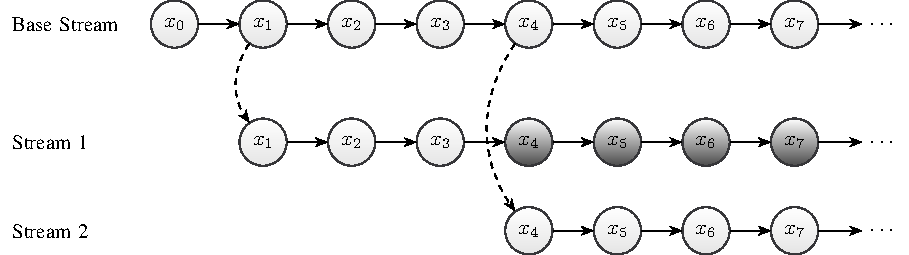
\includegraphics[width=0.95\textwidth]{figures/seeding_multiple_streams.pdf}
    \caption[Seeding Generation of Multiple Streams]{
      Generation of multiple streams by randomly seeding multiple instances of the same PRNG.
      Multiple instances of a full-period generator will cause overlapping subsequences.
    }
    \label{fig:seeding-multiple-streams}
  \end{figure}

  To use PRNGs for vectorized or parallelized algorithms, we have to provide multiple independent streams of random numbers.
  There are several methods to create and initialize such random streams.
  Exploiting vectorization facilities, usually multiple instances of the same generator which are seeded differently are used.
  For a full-period PRNG different seeds generate the same periodic part of a pseudorandom sequence starting at varying positions.
  Therefore the random initialization of all instances may cause the overlap of subsequences which is reducing statistical quality.
  Figure \ref{fig:seeding-multiple-streams} shows this overlap by means of an example.
  \autocite{fog2015,lecuyer2017}

  Some generators provide a so-called jumping routine that is able to advance the state of the PRNG by a large amount of steps.
  The Xoroshiro128+ for example makes it possible to discard $2^{64}$ or $2^{96}$ random numbers at once.
  Initializing multiple instances by using a jumping routine would guarantee non-overlapping subsequences with a length of the amount of random numbers discarded.
  \autocite{fog2015,lecuyer2017}

  \begin{figure}
    \center
    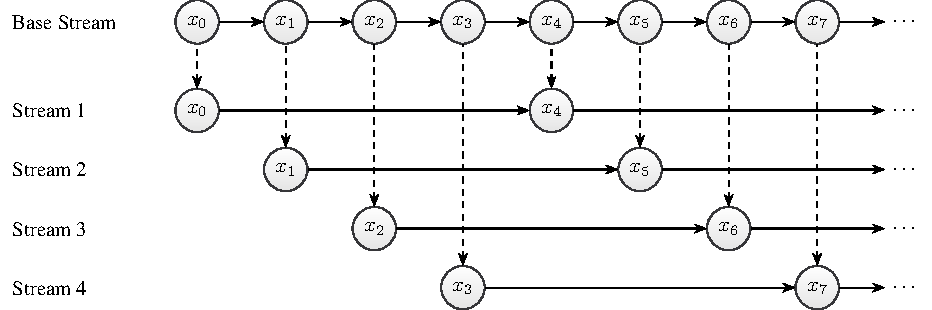
\includegraphics[width=0.95\textwidth]{figures/leapfrogging_multiple_streams.pdf}
    \caption[Leapfrogging Generation of Multiple Streams]{
      Generation of multiple streams by leapfrogging the output of a single PRNG instance.
      Consecutive values of a pseudorandom sequence will belong to different streams.
    }
    \label{fig:leapfrogging-multiple-streams}
  \end{figure}

  If the state of the generator is sufficiently large, only one instance would be used.
  Multiple streams are then constructed by the leafrogging method which can be seen in figure \ref{fig:leapfrogging-multiple-streams}.
  In this case, consecutive pseudorandom values will belong to different streams.
  \autocite{fog2015,lecuyer2017}


  % \subsection{Analyzation}
  % visualization, proof, experiments, benchmarks (runtime), test suites, code analyzation

  % statistical quality and performance vs implementation quality and performance

  % Visualizations: randograms 2d and 3d, histograms, simulation plots and images

  % Period and Uniformity, Empirical Testing, predictability and Security, Speed, Memory Size, Code Size, Output Range, Seekability, multiple streams, k-dimensional equidistribution, theoretical support, repeatability, portability, ease of implementation
  % subsection random_and_pseudorandom_number_generators (end)

  \subsection{Examples}
  \subsubsection*{Linear Congruential Generator} % (fold)
  % \label{ssub:linear_congruential_generator}
    A linear congruential Generator (LCG) is the most simplest example of an actual PRNG.
    The LCG uses modular arithmetic together with a simple recurrence relation.
    By carefully tweaking the parameters of the generator, enough randomness tests can be passed.
    \autocite{kneusel2018}

    \begin{definition}[Linear Congruential Generator]
      Let $m\in\setNatural$ with $m\geq 2$ and $a,c\in\setInteger_m$.
      We define the PRNG $\mathrm{LCG}(m,a,c) \define (S,T,U,G)$
      \[
        S \define U \define \setInteger_m
        \separate
        G \define \identity_{\setInteger_m}
      \]
      \[
        \function{T}{S}{S}
        \separate
        T(x) \define a x + c
      \]
      Multiplication and addition are understood in the sense of $\setInteger_m$.
      We call $\mathrm{LCG}(m,a,c)$ the linear congruential generator with modulus $m$, multiplier $a$ and increment $c$.
    \end{definition}
    If $c\neq 0$ then the LCG is non-linear and is able to provide equidistributed pseudorandom sequences with a maximum period of $m$.
    The generator function is the identity and therefore the LCG should not be used in more than one dimension.
    \autocite{kneusel2018}
  % subsection linear_congruential_generator (end)

  \subsubsection*{Mersenne Twister} % (fold)
  % \label{ssub:mersenne_twister}
    \begin{figure}
      \center
      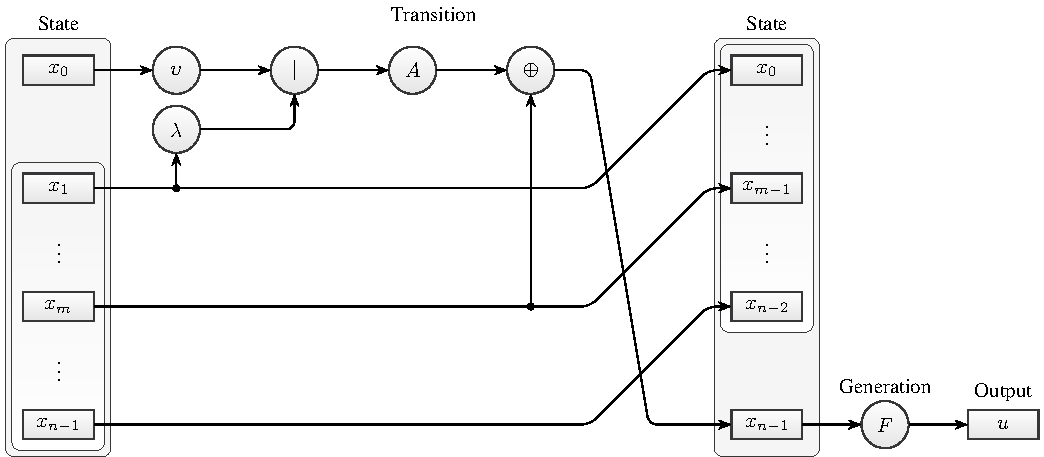
\includegraphics[width=0.95\textwidth]{figures/mt19937_scheme.pdf}
      \caption[Mersenne Twister Transition and Generation]{
        Transition and generator function of the Mersenne Twister.
        The notation is taken from definition \ref{def:mersenne-twister}.
      }
      \label{fig:mersenne-twister-transition-generation}
    \end{figure}

    The Mersenne twister is a linear PRNG with a maximum period of $2^{19937}-1$.
    Currently, it is the de facto standard when generating pseudorandom sequences.
    The mathematics behind the Mersenne twister are quite complex and we are not able to provide a rigorous introduction.
    But we will give an exact definition in the strict sense of a PRNG which was omitted in the original paper \autocite{matsumoto1998}.
    Additionally, figure \ref{fig:mersenne-twister-transition-generation} gives a schematic view of its transition and generator function.
    The generator was the first fast generator to produce 32-bit random numbers which exhibits 623-dimensional equidistribution and a high statistical quality.
    \autocite{kneusel2018}

    \begin{definition}[Mersenne Twister]
    \label{def:mersenne-twister}
      Let $w, n, m\in \setNatural$ and $r\in\setNatural_0$ with $m \leq n$ and $r < w$.
      Further, let $a,b,c \in \mathds{F}_2^w$ and $u,s,t,l \in \setInteger_w$.
      Then the Mersenne twister $\mathrm{MT}(w,n,m,r,a,b,c,u,s,t,l)\define (S,T,U,G)$ is defined as a PRNG in the following way.
      \[
        S \define \roundBrackets{\mathds{F}_2^w}^n
        \separate
        U \define \mathds{F}_2^w
      \]
      \[
        \function{T}{S}{S}
        \separate
        \function{G}{S}{U}
        \separate
        G(x) \define F(x_{n-1})
      \]
      For all $k\in\setNatural_0$ with $k < n-1$, we define $T$ as follows.
      \[
        T_k\roundBrackets{x} = x_{k+1}
        \separate
        T_{n-1}\roundBrackets{x} = x_{m} \oplus A\roundBrackets{υ(x_0) \,\middle\vert\, λ(x_{1})}
      \]
      Hereby, the following helper functions are used.
      \[
        \function{υ,λ}{\mathds{F}_2^w}{\mathds{F}_2^w}
      \]
      \[
        υ(x) = \underbrace{x_{w-1}\cdots x_r}_{w-r}\underbrace{0\cdots 0}_{r}
        \separate
        λ(x) = \underbrace{0\cdots 0}_{w-r}\underbrace{x_{r-1}\cdots x_0}_{r}
      \]
      \[
        \function{A}{\mathds{F}_2^w}{\mathds{F}_2^w}
        \separate
        A(x) \define
        \begin{cases}
          x \rightarrow 1 &: x_0 = 0 \\
          (x \rightarrow 1) \oplus a &: x_0 = 1
        \end{cases}
      \]
      \[
        \function{f_1,f_2,f_3,f_4}{\mathds{F}_2^w}{\mathds{F}_2^w}
      \]
      \begin{align*}
        f_1(x) &\define x \oplus (x \rightarrow u) &
        f_2(x) &\define x \oplus ((x \leftarrow s) \odot b) \\
        f_3(x) &\define x \oplus ((x \leftarrow t) \odot c) &
        f_4(x) &\define x \oplus (x \rightarrow l)
      \end{align*}
      \[
        \function{F}{\mathds{F}_2^w}{\mathds{F}_2^w}
        \separate
        F(x) \define f_4 \circ f_3 \circ f_2 \circ f_1(x)
      \]
      The Mersenne twister with the following parameters is called the MT19937.
      \begin{align*}
        w &= 32 & a &= \texttt{{0x9908b0df}} & u &= 11 \\
        n &= 624 & b &= \texttt{{0x9d2c5680}} & s &= 7 \\
        m &= 397 & c &= \texttt{{0xefc60000}} & t &= 15 \\
        r &= 31 & & & l &= 18
      \end{align*}
    \end{definition}
    % The state of the Mersenne Twister consists of 624 32-bit integers.

  % subsection mersenne_twister (end)

  % \subsection{Permuted Congruential Generator} % (fold)
  % \label{ssub:permuted_congruential_generator}
    % \begin{definition}[Permuted Congruential Generator]
    %   Given $\mathscr{G}\define \mathrm{LCG}(b,a,c)$ with transition function $T$.
    %   Let $t\in\setInteger_{b}$ and $\function{f_c}{\setInteger_{2^{b-t}}}{\setInteger_{2^{b-t}}}$ be a permutation for all $c \in \setInteger_{2^t}$.
    %   \[
    %     S \define \setInteger_{2^b}
    %     \separate
    %     U \define \setInteger_{2^{b-t}}
    %   \]
    %   \[
    %     G \define π_2 \circ f_* \circ \mathrm{split}_t
    %   \]
    %   \[
    %     f_*(a,b) \define (a,f_a(b))
    %   \]
    %   $\mathrm{PCG}(\mathscr{G},t,\set{f_c}{c\in\setInteger_{2^t}}) \define (S,T,U,G)$
    % \end{definition}
  % subsection permuted_congruential_generator (end)

  \subsubsection*{Xoroshiro128+} % (fold)
  % \label{ssub:xorshift_and_variants}
    \begin{figure}
      \center
      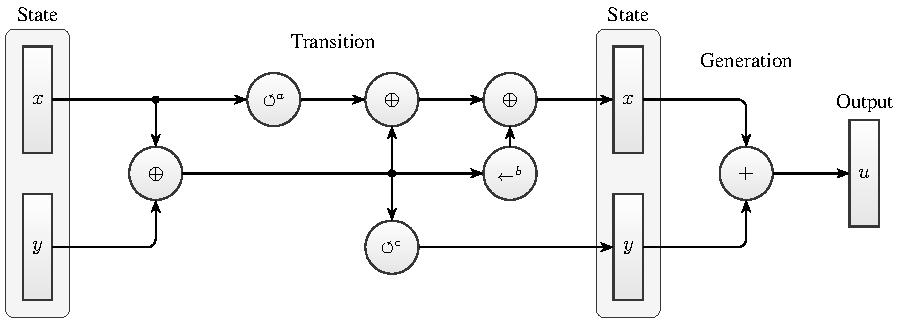
\includegraphics[width=0.95\textwidth]{figures/xrsr128p_scheme.pdf}
      \caption[Xoroshiro128+ Transition and Generation]{
        Transition and generation function of the Xoroshiro128+.
        The notation is taken from definition \ref{def:xoroshiro}.
      }
      \label{fig:xoroshiro-transition-generation}
    \end{figure}

    The Xoroshiro128+ is a scrambled linear PRNG with a maximum period of $2^{128}-1$.
    Figure \ref{fig:xoroshiro-transition-generation} visualizes its transition and generator function which are introduced in the following definition.
    Its state consists of two 64-bit integers that are interleaved by the use of different linear transformations when calling the transition function.
    The generator function scrambles the output through the use of a non-linear addition operation and returns a 64-bit integer.
    \autocite{kneusel2018,vigna-xoroshiro}

    \begin{definition}[Xoroshiro128+]
    \label{def:xoroshiro}
      Let $a,b,c \in \setInteger_{64}$.
      Then $\mathrm{Xoroshiro128+}(a,b,c)\define (S,T,U,G)$ is defined as a PRNG in the following way.
      \[
        S \define \roundBrackets{\mathds{F}_2^{64}}^2
        \separate
        U \define \mathds{F}_2^{64}
        \separate
        \function{T}{S}{S}
        \separate
        \function{G}{S}{U}
      \]
      \[
        T(x,y) \define (x \circlearrowleft a \oplus f(x,y) \oplus \boxBrackets{f(x,y) \leftarrow b},\ f(x,y) \circlearrowleft c)
      \]
      \[
        \function{f}{\mathds{F}_2^{64}}{\mathds{F}_2^{64}}
        \separate
        f(x,y) \define x \oplus y
      \]
      \[
        G(x,y) \define x + y
      \]
      If not otherwise stated, we assume $a=24$, $b=16$, and $c=37$.
    \end{definition}

  % subsection xorshift_and_variants (end)

  \subsubsection*{Middle Square Weyl Sequence RNG} % (fold)
  % \label{ssub:middle_square_weyl_sequence_rng}
    \begin{figure}
      \center
      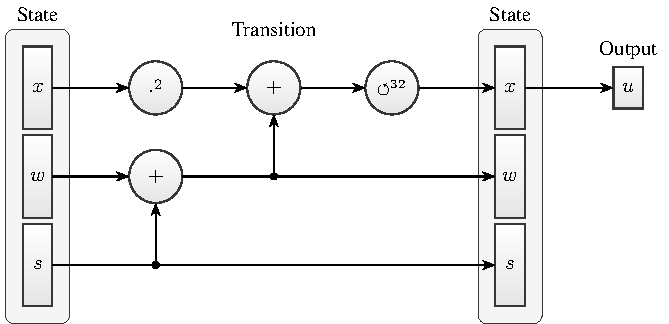
\includegraphics[width=0.7\textwidth]{figures/msws_scheme.pdf}
      \caption[Middle Square Weyl Sequence RNG Transition and Generation]{
        Transition and generation function of the middle square Weyl sequence RNG (MSWS).
        The notation is taken from definition \ref{def:msws}.
      }
      \label{fig:msws-transition-generation}
    \end{figure}

    The middle square Weyl sequence RNG (MSWS) is another modern generator which is based on a non-linear squaring routine in its transition function.
    It provides pseudorandom sequences of 32-bit integers with a period of $2^{64}$.
    In figure \ref{fig:msws-transition-generation}, again a schematic view of the transition and generator function is given.
    \autocite{widynski2019}

    \begin{definition}[Middle Square Weyl Sequence RNG (MSWS)]
    \label{def:msws}
      We define $\mathrm{MSWS}\define(S,T,U,G)$ as a PRNG in the following way.
      \[
        S \define \setInteger_{2^{64}}^3
        \separate
        U \define \setInteger_{2^{32}}
      \]
      \[
        \function{T}{S}{S}
        \separate
        T(x,w,s) = ((x^2 + w + s)\circlearrowleft 32, w+s, s)
      \]
      \[
        \function{G}{S}{U}
        \separate
        G(x,w,s) \define x \mod 2^{32}
      \]
    \end{definition}

  % subsection middle_square_weyl_sequence_rng (end)
% section pseudorandom_number_generators (end)
\end{document}